\documentclass[11pt,letterpaper]{article}
\usepackage[T1]{fontenc}
\usepackage{lmodern,microtype}
\usepackage[margin=.85in,headheight=15pt]{geometry}
\usepackage{xcolor,booktabs,longtable,array,tabularx,enumitem,amsmath,graphicx,listings,tikz,fancyhdr,titlesec,hyperref,xurl}
\usetikzlibrary{arrows.meta,positioning,fit,shapes.geometric}
\definecolor{navy}{HTML}{16314D}\definecolor{teal}{HTML}{087F83}\definecolor{pale}{HTML}{EDF4F8}\definecolor{muted}{HTML}{536579}
\hypersetup{colorlinks=true,linkcolor=navy,urlcolor=teal,pdftitle={Harness Engineering Technical Guide}}
\titleformat{\section}{\Large\bfseries\color{navy}}{\thesection}{.7em}{}
\titleformat{\subsection}{\large\bfseries\color{teal}}{\thesubsection}{.7em}{}
\pagestyle{fancy}\fancyhf{}\fancyhead[L]{\small Agent Harness Engineering}\fancyhead[R]{\small Technical study / v1.0}\fancyfoot[R]{\thepage}
\setlength{\parindent}{0pt}\setlength{\parskip}{5pt}\renewcommand{\arraystretch}{1.18}
\setlist{nosep,leftmargin=*}\newcolumntype{Y}{>{\raggedright\arraybackslash}X}
\newcommand{\src}[1]{\expandafter\nolinkurl\expandafter{\detokenize{#1}}}
\newcommand{\evidence}[1]{\par\smallskip{\small\raggedright\color{muted}\textbf{Source anchor:} #1\par}}
\tikzset{n/.style={draw=navy,rounded corners=2pt,fill=pale,align=center,minimum height=9mm,text width=31mm,font=\small},g/.style={n,draw=teal,fill=teal!7},edge/.style={-Latex,thick,draw=navy},boundary/.style={draw=teal,dashed,rounded corners,inner sep=5pt}}
\lstset{basicstyle=\small\ttfamily,breaklines=true,frame=single,backgroundcolor=\color{pale},columns=fullflexible,showstringspaces=false}
\begin{document}
\begin{titlepage}
\pagenumbering{roman}
\vspace*{1.25in}
{\color{teal}\large AGENT HARNESS COURSE STUDY / 02\par}\vspace{.3in}
{\color{navy}\Huge\bfseries Harness Engineering Technical Guide\par}\vspace{.18in}
{\Large Practical operating reference, diagrams and verification\par}\vspace{.5in}
\rule{\linewidth}{1pt}\par
\textbf{Source:} Richmond Alake's Harness Engineering for AI Agents course export\par
\textbf{Version:} 1.0 \quad 23 November 2026\par
\textbf{Status:} Technical study; not a production authorization\par
\vfill
The model proposes; the harness validates, governs, executes and records.
\end{titlepage}
\pagenumbering{arabic}
\tableofcontents\clearpage
\section*{Reading note}
This standalone volume belongs to a six-document study of snapshot \src{8a5edab282632443}. Observed source behavior is distinguished from proposed controls. No live application, external provider or sandbox was independently executed. Test files are contract evidence, not independently verified passing results.

\section{Purpose and operating profiles}
This guide is a practical companion to the separate architecture analysis. Use a full upstream checkout for experiments, not the supplied text export. Begin with credential-free practice data and scripted responders. Install only the dependencies required by the chosen part. The documented commands below were inspected in the course snapshot; execution has not been independently reproduced.
\begin{tabularx}{\linewidth}{p{.22\linewidth}YY}\toprule
Profile & Entry point & Interpretation \\\midrule
ERPA packaged & Part 1 MemoRizz appbook, port 8000 & Compare bundled memory and tool abstractions \\
ERPA custom & Part 1 custom appbook, port 8001 when overridden & Inspect staged construction and trace \\
PPA Part 2 & Custom appbook, port 8020 & Practice workspace; gateway on 8941 \\
PPA Part 3 & Custom appbook, port 8050 & Separate gateway on 8951; cost, trajectories, learning \\
Research & Part 3 research appbook, port 8041 & Live prerequisites; outline and publication gates \\
\bottomrule\end{tabularx}
\section{Local setup and first run}
From the course root, create a Python 3.11+ virtual environment and install the two Part 1 appbook requirement sets. Inspect dependency pins first. The installation command requires package access; subsequent scripted exercises need no provider account.
\begin{lstlisting}[language=bash]
python -m venv .venv
source .venv/bin/activate
python -m pip install \
  -r part_1/harness_done_for_you/memorizz/assistant/appbook/requirements.txt \
  -r part_1/custom_harness/appbook/requirements.txt
python part_1/tests/smoke_test.py
\end{lstlisting}
Run the six independent stages from the root. Compare adjacent files to identify what changed rather than treating a successful response as proof of architecture.
\begin{lstlisting}
python part_1/custom_harness/stages/stage_01_single_turn.py
python part_1/custom_harness/stages/stage_02_memory.py
python part_1/custom_harness/stages/stage_03_semantic_layer.py
python part_1/custom_harness/stages/stage_04_skills.py
python part_1/custom_harness/stages/stage_05_tools.py
python part_1/custom_harness/stages/stage_06_complete_harness.py
\end{lstlisting}
\begin{lstlisting}
cd part_1/custom_harness/appbook
PORT=8001 ./run.sh
\end{lstlisting}
In a separate terminal from the repository root, run PPA Part 2 or Part 3. Do not reuse a data directory or assume provider keys are absent merely because the UI shows practice data.
\begin{lstlisting}
cd part_3/custom_harness
python -m venv .venv
.venv/bin/python -m pip install -r appbook/requirements.txt
cd appbook
PPA_RESPONDER=scripted ./run.sh
\end{lstlisting}
Inspect the responder label, workspace mode and tracing setting before entering data. Leave live accounts disconnected, remove unused provider keys from the environment and disable external tracing for private experiments. Part 3 has no UI form for real-account connections but its gateway retains endpoints; this is not a security boundary.
\evidence{\src{README.md}; \src{part_1/custom_harness/stages/README.md}; \src{part_2/custom_harness/appbook/README.md}; \src{part_3/custom_harness/appbook/README.md}.}
\section{Inspecting a turn}
\begin{enumerate}
\item Submit a fixture question and identify the request, context layers and selected tool before examining the answer.
\item Inspect the tool schema, host decision, result and run trace. Compare automatic reads with a drafted mock outward effect.
\item Reject the draft, confirm it was not delivered, and inspect the persisted action log. Repeat with an allowed practice effect.
\item Start a focus timer or scheduled routine in the practice workspace and inspect its state independently of the conversational turn.
\item Compare fresh sessions, memory recall and scratch promotion; identify what was retained and why.
\item In Part 3 inspect the cost ledger and trajectory, then a candidate skill gate and scorecard. Scripted zero cost is not a measurement of live-provider cost.
\end{enumerate}
\section{Live and advanced tracks}
Live operation is optional and requires explicit approval of data transfers, credentials, provider quotas, persistence, network access and cost. Part 1 advanced requirements and tests are documented as follows:
\begin{lstlisting}
.venv/bin/python -m pip install --upgrade -r part_1/advanced/requirements.txt
.venv/bin/python -m pytest -q part_1/advanced/tests
\end{lstlisting}
Part 3 research requires Docker, Anthropic and Tavily credentials and can start Oracle locally. Its documented default model budget is six dollars per paper; configuration and actual cost must be checked before each live run. The research workflow pauses for outline and publication review. Record checkpoints and evidence; do not publish without independent review. A documented command is not permission to execute it.
\evidence{\src{part_1/advanced/README.md}; \src{part_3/advanced/deep_research/appbook/README.md}.}
\section{Troubleshooting and verification}
\begin{longtable}{>{\raggedright\arraybackslash}p{.27\linewidth}>{\raggedright\arraybackslash}p{.64\linewidth}}\toprule
Symptom & Diagnostic and expected result \\\midrule\endhead
Import error & Check the active interpreter and selected requirements; do not install unrelated provider packages indiscriminately. \\
Gateway unavailable & Inspect health, process logs and configured local port; do not bypass gateway authentication. \\
Unexpected live calls & Check responder, environment and tracing flags; stop the run and remove unnecessary keys. \\
Zero usage cost & Confirm scripted responder; do not infer provider caching performance. \\
No retrieval result & Inspect fixture/source provenance, scope and cache before enlarging access. \\
Run waiting & Inspect checkpoint and approval state; do not repeatedly approve or retry a possibly delivered effect. \\
Blocked scorecard & Inspect each mandatory criterion; missing evidence is not a pass. \\
\bottomrule\end{longtable}
Record source revision, Python and dependency versions, run ID, mode, test output, trace and sanitized screenshots. A successful local demonstration proves only the tested fixture behavior. Review the security assessment before connecting real systems.

\section{Control-flow reference}
\subsection{Turn lifecycle and data flows}
Part 3's \src{agent.py} assembles context, calls the model, dispatches validated tools, drafts effects, interrupts at human review, applies effects, calls the model again, and persists. Automatic tools and gated tools follow distinct paths. Approval decisions are written separately from delivery results. In contrast to Part 1's repeated context assembly, Part 3 aims to assemble stable context once and track provider prompt caching. The graph checkpoint is not itself a transaction with external mail or calendar services.
\begin{center}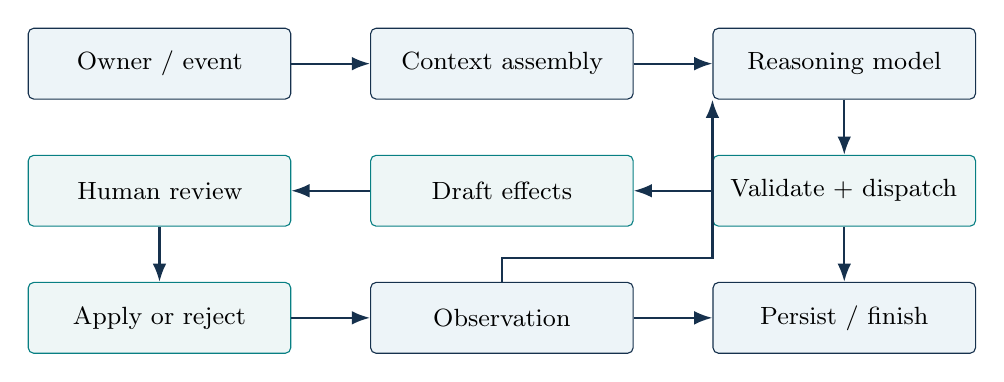
\begin{tikzpicture}[node distance=7mm and 10mm]
\node[n] (req) {Owner / event};\node[n,right=of req] (ctx) {Context assembly};\node[n,right=of ctx] (model) {Reasoning model};
\node[g,below=of model] (disp) {Validate + dispatch};\node[g,left=of disp] (draft) {Draft effects};\node[g,left=of draft] (review) {Human review};
\node[g,below=of review] (apply) {Apply or reject};\node[n,right=of apply] (obs) {Observation};\node[n,right=of obs] (persist) {Persist / finish};
\draw[edge](req)--(ctx);\draw[edge](ctx)--(model);\draw[edge](model)--(disp);\draw[edge](disp)--(draft);\draw[edge](draft)--(review);\draw[edge](review)--(apply);\draw[edge](apply)--(obs);\draw[edge](disp)--(persist);\draw[edge](obs)--(persist);\draw[edge](obs.north)--++(0,3mm)-|(model.south west);
\end{tikzpicture}\end{center}
\textit{Figure 1. Logical turn flow. The observation is supplied to the model for another bounded iteration; persistence may occur at checkpoints and on termination. The direct dispatch-to-persist edge summarizes the automatic/final path, not an exact graph edge.}
\subsection{Memory and context engineering}
\begin{tabularx}{\linewidth}{p{.23\linewidth}YY}\toprule
Memory & Content & Required lifecycle \\\midrule
Working & Current scratch, task plan, context window & Session-scoped, bounded, expires \\
Episodic & Past interactions and outcomes & Owner-scoped, redacted, time-stamped \\
Semantic & Facts, evidence, domain meaning & Provenance, freshness, conflict handling \\
Procedural & Skills and workflow recipes & Immutable versions, review and rollback \\
\bottomrule\end{tabularx}

The course uses scratch working memory and promotion to longer-term stores, with content-hash deduplication described in the PPA appbook. Distinguish raw evidence from extracted claims and approved instructions. Retrieval selects candidates, reranks and builds a bounded context; it never grants authority. Semantic cache hits are not prompt-cache hits: the former reuse a previous answer based on matching semantics, the latter reuse provider computation over a stable prefix. Never reuse authorization decisions, private data across principals, or an effectful completion on semantic similarity alone. The proposed cache key includes tenant, principal/scope, source versions, policy version, skill revision and model configuration; effectful requests bypass answer reuse.
\evidence{Part 1 \src{cache.py}, \src{retriever.py}, \src{semantic.py}; Part 3 \src{scratchfs.py}, \src{memory.py}, \src{ledger.py}.}
\subsection{Advanced modes}
The Part 1 advanced workflow documents a 17-node graph with missing-evidence, quick and parallel high-risk branches, Oracle checkpointing, semantic tool and skill registries and workflow promotion. The research track uses six MemAgents, private/shared Oracle memory, Tavily retrieval and governed E2B execution. The MetaHarness normalizes runs across model wrappers and records evidence; the separate fair evaluation notebook controls task samples and provider differences. Total Recall adds ontology/GraphRAG and governed semantic registries. These are documented implementations, not verified external services.

Part 3 research is a separate graph, not simply the assistant with a longer prompt. Its \src{graph.py} scopes a paper, interrupts for outline approval, gathers evidence, tallies, reflects, organizes, fans out writing, reviews, assembles and interrupts for publication review. Reflection is constrained by thin evidence, remaining rounds, new sources and budget. A blocked release permits an explicit override in source; production should restrict override authorization and record justification, or prohibit it for hard safety failures.
\begin{center}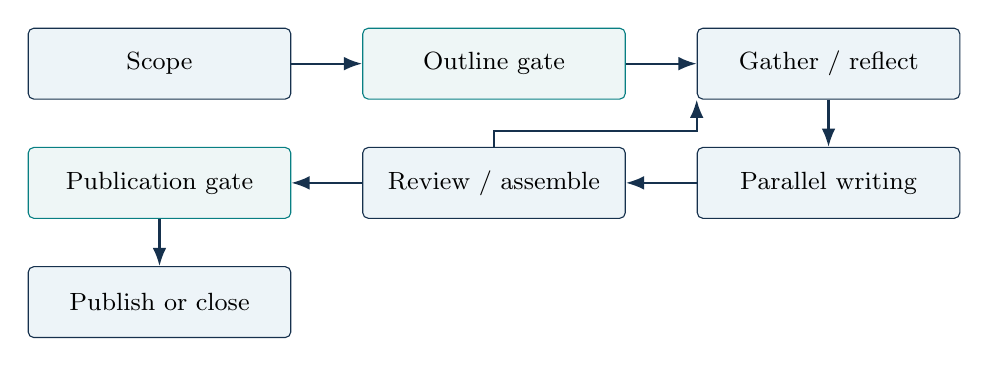
\begin{tikzpicture}[node distance=6mm and 9mm]
\node[n] (s) {Scope};\node[g,right=of s] (a) {Outline gate};\node[n,right=of a] (r) {Gather / reflect};\node[n,below=of r] (w) {Parallel writing};\node[n,left=of w] (v) {Review / assemble};\node[g,left=of v] (p) {Publication gate};\node[n,below=of p] (o) {Publish or close};
\draw[edge](s)--(a);\draw[edge](a)--(r);\draw[edge](r)--(w);\draw[edge](w)--(v);\draw[edge](v)--(p);\draw[edge](p)--(o);\draw[edge](v.north)--++(0,2mm)-|(r.south west);
\end{tikzpicture}\end{center}
\evidence{\src{part_1/advanced/README.md}; \src{part_1/advanced/INSTRUCTOR_RUNBOOK.md}; \src{part_3/advanced/deep_research/appbook/backend/harness/graph.py}, \src{budget.py}, \src{evidence.py}.}
\section{Source register and limitations}
\begin{itemize}
\item Richmond Alake, \textit{Harness Engineering for AI Agents}, supplied repository export,\newline snapshot \src{8a5edab282632443}; root README, Part 1--3 READMEs, code paths cited throughout. Workshop: \url{https://www.oreilly.com/live-events/harness-engineering-for-ai-agents/0642572381264}.
\item Target curriculum, README and roadmap, inspected 23 November 2026: \url{https://github.com/Notoriousjayy/agent-engineering-curriculum}.
\item Target documentation library, root README and AI technical-documents directory, inspected 23 November 2026: \url{https://github.com/Notoriousjayy/latex-docs}.
\end{itemize}
All figures are original logical reconstructions or proposed design diagrams; they are not copies of source graphics. Vendor-neutral controls, ADRs, acceptance tests and laboratory extensions are recommendations rather than claims about source implementation. Live dependencies, source test outcomes, provider claims, licensing/publication clearance and deployment configuration require separate validation.
\end{document}
